\documentclass{magnolia}

\magtex{tex_driver={pdftex}}
\magfiche{document_nom={Flot d'exécution},
          auteur_nom={François Fayard},
          auteur_mail={francois.fayard@auxlazaristeslasalle.fr}}
\magcours{cours_matiere={maths},
          cours_niveau={mpsi},
          cours_chapitre_numero={1},
          cours_chapitre={Flot d'exécution}}
\magmisenpage{}
\maglieudiff{}
\magprocess

\begin{document}

%BEGIN_BOOK

\section{Altimètre}
Un altimètre est un instrument de mesure permettant de déterminer la distance verticale entre un
point et une hauteur de référence. Lors d'une randonnée en montagne, Max étalonne son altimètre
à son point de départ, puis mesure à chaque heure l'altitude relative atteinte. À la fin de sa
randonnée, il obtient une liste d'entiers naturels qu'il range dans une liste Python 
\verb!alt = [0, 300, 500, 600, 1000, 800, 900, 500, 600, 200, 0]!. 

\begin{center}
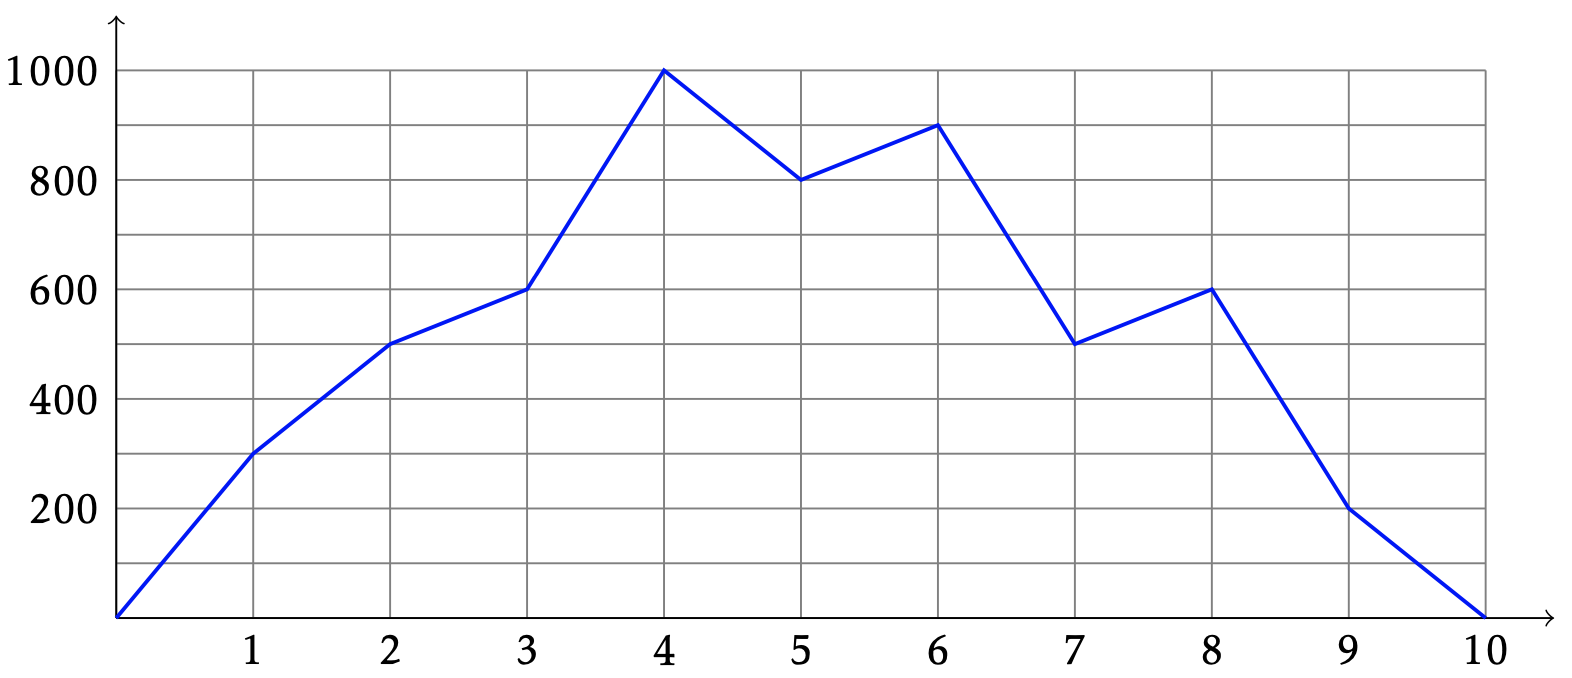
\includegraphics[width=0.65\textwidth]{../../Commun/Images/python-tp-altimetre}\\
\textsc{Figure 1} -- La randonnée de Max a duré 10 heures, il a atteint une
altitude relative\\ de 300~m au bout d'une heure, de 500~m au bout de deux heures, etc.
\end{center}

Max souhaite maintenant calculer certaines valeurs relatives à son parcours.

\begin{questions}
\question Comment obtenir la durée de la randonnée~? 
\question Définir en Python une fonction \verb!altmax(alt: list[int]) -> int!, qui prend en argument
  une liste \verb!alt! et qui renvoie l'altitude relative maximale atteinte lors de sa randonnée. Par
  exemple, dans le cas de l'illustration numérique donnée ci-dessus, la fonction devra renvoyer la
  valeur 1000.
\enonce Max cherche maintenant à savoir à quel moment son ascension a été la plus rapide en
  calculant le dénivelé maximal réalisé en une heure. Dans toute la suite de l'exercice,
  le dénivelé dont nous parlons est le dénivelé algébrique, qui est positif lorsque Max
  monte et négatif lorsque Max descend.  Il cherche donc la plus grande différence
  entre deux emplacements consécutifs de la liste. Par exemple, pour la liste donnée en illustration,
  le dénivelé maximal est égal à 400 et a été réalisé entre la troisième et la quatrième heure.
\question Définir en Python une fonction baptisée \verb!deniv_max(alt: list[int]) -> int! prenant
  en argument une liste \verb!alt! et renvoyant le dénivelé maximal réalisé en une heure durant
  sa randonnée. 
\question Écrire une fonction \verb!heure_deniv_max(alt: list[int]) -> int! renvoyant l'heure
  à laquelle débute la réalisation de ce dénivelé. Pour la liste donnée en exemple, cette fonction
  devra donc renvoyer la valeur 3.
\question Définir une fonction \verb!deniv_positif_total(alt: list[int]) -> int! renvoyant la somme des
  dénivelés positifs réalisés durant cette randonnée. Pour l'exemple donné en illustration, cette
  fonction devra renvoyer la valeur 1200.
\enonce Enfin, on appelle \emph{sommet} tout point dont l'altitude relative est strictement supérieure à
  l'altitude qu'elle précède et à l'altitude qui lui succède dans la liste \verb!alt!. Dans
  l'exemple qui nous sert à illustrer cet exercice, la randonnée de Max présente trois
  sommets d'altitudes 1000, 900 et 600 atteints à la quatrième, sixième et huitième heure de
  marche.
\question Écrire une fonction \verb!sommets(alt: list[int]) -> NoneType! affichant les
  différentes heures et altitudes des sommets de la randonnée.
\end{questions}

\section{La conjecture de Syracuse}

On doit cette conjecture au mathématicien allemand Lothar Collatz qui, en 1937, proposa à la
communauté mathématique le problème suivant~:\\

\parbox[c]{0.92\linewidth}{\emph{On part d'un nombre entier strictement positif. S'il est pair,
on le divise par 2. S'il est impair, on le multiplie par 3 et on ajoute 1. On réitère ensuite
cette opération.}}\\

Par exemple, à partir de 14 on construit la suite de nombres~: 14, 7, 22, 11, 34, 17, 52, 26,
13, 40, 20, 10, 5, 16, 8, 4, 2, 1, 4, 2, 1, etc. Après que le nombre 1 ait été atteint, la suite
des valeurs 4, 2, 1 se répète indéfiniment en un cycle de longueur 3.

\begin{center}
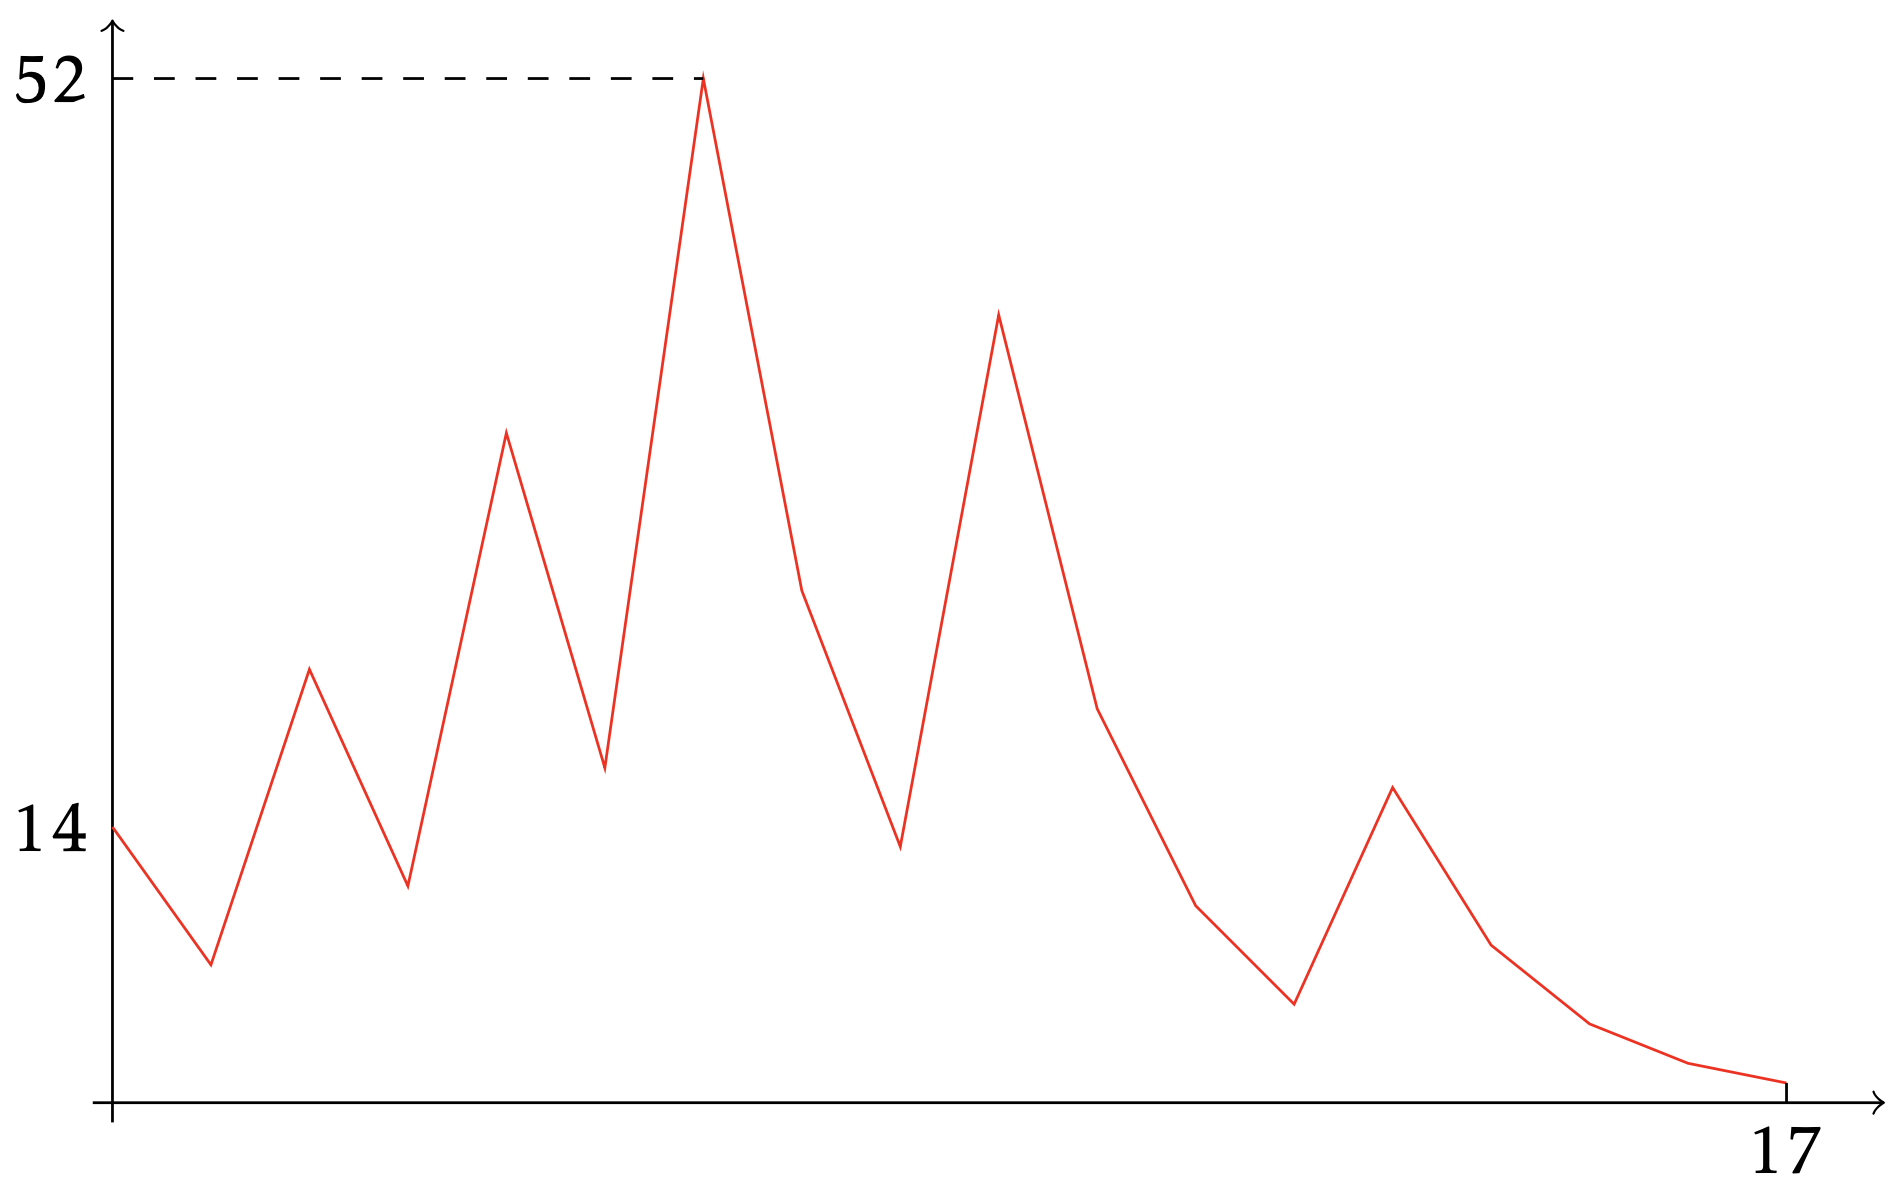
\includegraphics[width=0.45\textwidth]{../../Commun/Images/python-tp-collatz}\\
\textsc{Figure 2} -- Le graphe de la suite de Collatz pour $c=14$
\end{center}

La conjecture de Syracuse est l'hypothèse mathématique selon laquelle n'importe quel entier
de départ conduit à la valeur 1 au bout d'un certain temps. Nous allons expérimenter cette
conjecture en programmant l'évolution de la suite $(u_n)$ définie par les relations
\[u_0\defeq c\qquad\text{et}\qquad \forall n\in\N\qsep
  u_{n+1}=\begin{cases}\frac{u_n}{2} & \text{si $u_n$ est pair,}\\ 3u_n+1 & \text{si $u_n$ est impair.}\end{cases}\]

\subsection{Temps de vol et altitude maximale}

\begin{questions}
\question Écrire une fonction \verb!f(u: int) -> int! prenant en entrée un entier $u$ et renvoyant
  $u/2$ si $u$ est pair et $3u+1$ si $u$ est impair.
\enonce Le \emph{temps de vol} d'un entier $c$ est le plus petit entier $n$ (en admettant qu'il existe) pour lequel
  $u_n=1$. Par exemple, le temps de vol pour $c=14$ est égal à 17.
\question Définir une fonction \verb!temps_de_vol(c: int) -> int! prenant un paramètre entier $c$ et renvoyant
  le plus petit entier $n$ pour lequel $u_n=1$.
\enonce De manière tout aussi imagée, on appelle \emph{altitude maximale} de $c$ la valeur maximale de la suite $(u_n)$.
  Par exemple, l'altitude maximale de $c=14$ est égale à 52.
\question Écrire une fonction \verb!altitude(c: int) -> int! qui calcule cette fois-ci l'altitude maximale pour un
  entier $c$ donné en paramètre.
\end{questions}

\subsection{Vérification expérimentale de la conjecture}

On désire désormais vérifier la validité de la conjecture pour toute valeur $c\leq 1\ 000\ 000$. Une première solution
consisterait à calculer le temps de vol pour toutes ces valeurs, mais ce calcul est long et il y a mieux à faire en
observant que si la conjecture a déjà été vérifiée pour toute valeur $c'<c$, il suffit qu'il existe un rang $n$ pour
lequel $u_n<c$ pour être certain que la conjecture sera aussi vérifiée au rang $c$. On appelle donc
\emph{temps d'arrêt} le premier entier $n$ (en admettant qu'il existe) pour lequel $u_n<c$.

\begin{questions}
\question Écrire une fonction \verb!temps_d_arret(c: int) -> int! prenant un paramètre entier $c$ et renvoyant le temps
  d'arrêt de la suite de Syracuse correspondante.
\enonce Nous souhaitons maintenant mesurer le temps nécessaire pour vérifier la conjecture jusqu'à un paramètre entier
  $m$. Pour cela, nous allons utiliser la fonction \verb!time! du module \verb!time! du même nom, sans argument, qui
  renvoie le temps en secondes depuis une date de référence (qui dépend du système).
\question À l'aide de cette fonction, écrire une fonction \verb!verification(m: int) -> float! qui prend en argument
  un entier $m$ et renvoie le temps nécessaire pour vérifier que toutes les valeurs de $c\in\intere{2}{m}$ ont bien
  un temps d'arrêt fini. Quelle durée d'exécution obtient-on pour $m=1\ 000\ 000$~?
\question Quel est le temps d'arrêt d'un entier pair~? d'un entier de la forme $c=4n+1$~? En déduire qu'on peut restreindre
  la recherche aux entiers de la forme $4n+3$ et modifier en conséquence la fonction précédente. Combien de temps
  gagne-t-on par rapport à la version précédente pour $m=1\ 000\ 000$~? Vérifier ensuite la conjecture pour
  $n=10\ 000\ 000$.
\end{questions}

\subsection{Records}

\begin{questions}
\question Déterminer l'altitude maximale que l'on peut atteindre lorsque $c\in\intere{1}{1\ 000\ 000}$, ainsi que la
  valeur minimale de $c$ permettant d'obtenir cette altitude.
\question Déterminer le temps d'arrêt maximal lorsque $c\in\intere{1}{1\ 000\ 000}$ ainsi que la valeur de $c$
  correspondante.
\enonce On appelle \emph{vol en altitude de durée record} un vol dont tous les temps d'arrêt de rangs inférieurs
  sont plus courts. Par exemple, le vol réalisé pour $c=7$ est un vol en altitude de durée record (égale à 11)
  car tous les vols débutant par $c=1, 2, 3, 4, 5, 6$ ont des temps d'arrêt de durées inférieures à 11.
\question Déterminez tous les vols en altitude de durée record pour $c\leq 1\ 000\ 000$.
\end{questions}

\subsection{Affichage du vol}

Pour obtenir des graphes analogues à celui de la figure 2, on utilise la fonction \verb!plot! qui appartient à
un module appelé \verb!matplotlib.pyplot! et dédié au tracé des graphes. Vous allez donc commencer par importer
celui-ci à l'aide de la commande

\begin{pythoncode}
import matplotlib.pyplot as plt
\end{pythoncode}

Désormais, toutes les fonctions de ce module vous sont accessibles à condition de les préfixer par \verb!plt!.
Nous n'aurons besoin aujourd'hui que de deux fonctions \verb!plt.plot! et \verb!plt.show!. Sous sa forme la plus
simple, la fonction \verb!plt.plot! n'exige qu'une liste en paramètre \verb!plt.plot([a0, a1, ..., an])! et
crée un graphe constitué d'une ligne brisée reliant les points de coordonnées $(k,a_k)$ pour $k\in\intere{0}{n}$.
En Python, une liste est encadrée par des crochets et ses éléments sont séparés par des virgules. Nous étudierons
les listes plus tard dans le cours, mais pour l'instant nous n'aurons que besoin du fait que \verb![]! représente la liste
vide et si \verb!lst! est une liste, on ajoute un élément à la fin de celle-ci à l'aide de la commande
\verb!lst.append(x)!. Une fois votre graphe créé par la fonction \verb!plt.plot!, il reste à le faire
apparaitre dans une fenêtre annexe à l'aide de l'instruction \verb!plt.show()!.

\begin{questions}
\question Définir une fonction \verb!graphique(c: int) -> NoneType! qui prend un entier $c$ en paramètre et
  qui construit le graphe de la suite $(u_n)$ durant son temps de vol.
\end{questions}

\subsection{Encore une optimisation}

Nous avons vu plus haut qu'il suffit de restreindre l'étude de la conjecture aux entiers de la forme $4n+3$,
soit à $25\%$ des entiers. On peut chercher à affiner cette démarche en s'intéressant aux entiers de la forme
$8n+k$ mais ceci ne conduit pas à une amélioration des performances puisqu'on ne peut que restreindre l'étude
aux entiers de la forme $8n+3$ et $8n+7$. En revanche, il est possible de restreindre l'étude aux entiers
de la forme $16n+7$, $16n+11$ et $16n+15$, soit $18.75\%$ des entiers.

\begin{questions}
\question Si on écrit les entiers sous la forme $65536n+k$ ($65536=2^{16}$), à combien de valeurs de $k$
peut-on restreindre l'étude~?
\end{questions}
%END_BOOK
\end{document}